\documentclass{article}

% if you need to pass options to natbib, use, e.g.:
%     \PassOptionsToPackage{numbers, compress}{natbib}
% before loading neurips_2020

% ready for submission
% \usepackage{neurips_2020}

% to compile a preprint version, e.g., for submission to arXiv, add add the
% [preprint] option:
\usepackage[preprint]{neurips_2022}

% to compile a camera-ready version, add the [final] option, e.g.:
%     \usepackage[final]{neurips_2020}

% to avoid loading the natbib package, add option nonatbib:
%\usepackage[nonatbib]{neurips_2020}

\usepackage[utf8]{inputenc} % allow utf-8 input
\usepackage[T1]{fontenc}    % use 8-bit T1 fonts
\usepackage{hyperref}       % hyperlinks
\usepackage{url}            % simple URL typesetting
\usepackage{booktabs}       % professional-quality tables
\usepackage{amsfonts}       % blackboard math symbols
\usepackage{nicefrac}       % compact symbols for 1/2, etc.
\usepackage{microtype}      % microtypography
\usepackage{graphicx}       % to compile images

\title{Methods for Stratego AI}

\author{%
  Iain~Found\\
  School of Computer Science\\
  Carleton University\\
  Ottawa, ON, K1S 5B6 \\
  \texttt{iainfound@cmail.carleton.ca} \\
  \And
  Henry~Zhangxiao\\
  School of Computer Science\\
  Carleton University\\
  Ottawa, ON, K1S 5B6 \\
  \texttt{henryzhangxiao@cmail.carleton.ca} \\
}

\begin{document}

\maketitle

\begin{abstract}
% Dummy text, put a real abstract here
Stratego is an information incomplete board game with a possible $10^{66}$ starting arrangements for any new Stratego game and a game tree complexity of $10^{535}$, far exceeding the complexity of any other board game.
What separates novice level naïvely implemented Stratego bots from human players is the evaluation of the need to perform computations on a particular board state, as well as the introduction of playstyle variability and bluffing.
In this paper, we will touch upon five algorithms and their implementations which use varying methods in their setups and executions, as well as their limitations.
\end{abstract}

\section{Data-Based Stratego Bots }

One realm of Stratego reinforcement learning relies on the data it gathers from the opponent as well as the environment.
Due to the incomplete information nature of Stratego, one of the aspirations for a data-based algorithm is to explore the unknown grid-map while constantly assessing the risk.
Expolaratory Stratego bots must also use the information it derives from the playstyle of the opponent to gain an edge in strategical planning.

\subsection{Probabilistic Multi-ply Multi-Agent}

Using probabilities and Bayesian networks, Stankicwicz has focused on opponent modelling [1] to determine the rank of each piece, based on previous games with the same opponent. 
The simulated behaviour of the opponent was also considered. A probability distribution is attached to each piece to simulate the behaviour. 
Modelling the opponent led to correct rank prediction 40\% of the time, compared to only 18\% in case of not using opponent modelling. 
This higher prediction has led to a 55\% win rate against the opponent without the model of the other player.

\subsubsection{Probabilistic Agent}

The probabilistic agent evaluates the outcome of all next legal moves and picks the best one. 
The best move is given by an evaluation function. Since the number of each piece type of the enemy is known, the probabilistic agent stores a table with scores with the remaining pieces. 
The number of pieces of a particular rank will be associated with that rank in the table. 
The probability of the agent to choose the rank \textit{r} for the attacked piece of colour \textit{c} $\in$ \{blue,red\} is defined as 
$$ p_r^c = \frac{i_r}{\sum_{s \in R^c}{i_s}} , \forall r \in R^c $$ where \textit{$i_r$} is the number of pieces of rank \textit{r}, the denominator is the number of remaining pieces of the enemy, 
\textit{$R^c$} is the set of all ranks of the pieces the enemy has on the board. However, if it is known that the attacked piece of the enemy was moved, then the immobile pieces are not considered anymore: 
$$ p_{r_m}^c = \frac{i_{r_m}}{\sum_{s \in R^c_m}{i_s}} , \forall r_m \in R^c_m $$ where $R^c_m$ is the set of the ranks of the movable pieces the enemy has left on the board, which leads to: $R^{player}_m$ = $R^{player}$\textbackslash\{F,B\}. 

\subsubsection{Muti-ply Agent}

Similar to the probabilistic agent, for each legal move, the agent chooses a rank for the attacked piece if there is an attacked piece of unknown rank. 
Different from the probabilistic agent is that instead of evaluating the resulting position immediately for each move, the multi-ply agent simulates the next moves of the opponent. 
For this, the player generates a possible game position for the enemy, that is consistent with the information currently known about the opponent. 
Then it uses the information that it knows the opponent certainly knows about it for keeping the consistency in the newly simulated position. 
Similarly with the probabilistic agent, the multi-ply agent evaluates the resulting position next and chooses the best move. 
For simulating the opponent’s move, the agent considers if the other agent is a probabilistic or a multi-ply one. 

\subsubsection{Results with Different Configurations}

The agents are compared in Table I, where \textit{total} represents the number of played games. 
Here, \textit{VR} represents red victories as a percentage of the total, \textit{VRC} are red victories with capture, as a percentage of \textit{VR}. 
Similarly, \textit{VA} are blue victories as a percentage of the total number of games, while \textit{VAC} are blue victories with capture, as a percentage of \textit{VR}. 
The execution time is denoted with \textit{$t_e$}. Two evaluation functions were used: basic evaluation function \textit{fb} and material evaluation function \textit{fm}. 
The players use the same configuration for the starting position. [3] 

\begin{table}
  \caption{Comparing Agents using Different Parameters with the Same Setup [1]}
  \label{multi-agent-results}
  \centering
  \begin{tabular}{ccccccccc}
  \#E     &red(R) & blue(A) & VR\% & VRC\% & VA\% & VAC\% & total & $t_e(m)$  \\
  \toprule
    1			& random	& probabilistic, \textit{fm}	& 1.4\%	              & 75.1\%  & 98.5\% & 0\%      & 10,000  & 4\\
    2	    & random	& probabilistic, \textit{fb}	& 10.2\%	            & 10.4\%  & 89.7\% & 34.27\%  & 10,000  & 4\\
    3     & random	& 2-ply, \textit{fb}	        & 14.5\%	            & 16.5\%  & 85.5\% & 55.7\%   & 1,000   & 8\\
    4			& random	& 3-ply, \textit{fb}	        & 16\%	              & 6.25\%  & 84\%   & 76.1\%   & 100     & 21\\
    5			& probabilistic, \textit{fb}	& 3-ply, \textit{fb}	& 41.1\%	&42.1\%   & 58.8\% & 87.5\%   & 450     & 79\\
    \bottomrule
  \end{tabular}
\end{table}

\subsection{Invincible - A Stratego Bot}

“Invincible” uses original approaches for creating setups, making guesses about the ranks of unknown pieces and reasoning about the best move in a given situation. [2] 
Setups are created by a combination of statistical information of human-created setups and heuristic evaluation of the results to select the best of a number of semi-random setups. 
The basis of “Invincible” is a collection of plans that give a value to every possible move. The move with the highest total contribution to all the plans is selected. 
These plans evaluate only a single ply, so no deeper searches are made. 
Since plans have a well-defined goal, the complexity of finding how well a move contributes to a plan is usually constant, or at most dependent on the (constant) size of the board. 

The advantages and disadvantages of using a plan-based algorithm:

\begin{itemize}
  \item Advantages:
  \begin{itemize}
    \item “Unlimited” search depth (4.1).
    \item Possibilities to bluff (4.2).
    \item Possibilities to coordinate attacks with multiple pieces. (4.3).
    \item Focus computation on interesting situations. (4.4).
  \end{itemize}
  \item Disadvantages:
  \begin{itemize}
    \item “Invincible” knows only what it’s told (4.5).
    \item Comparable information is calculated multiple times (4.6).
    \item Game specific knowledge needed (4.7).
  \end{itemize}
\end{itemize}

\subsubsection{Plans}

In particular, plans can see: The current board with the position of all the pieces, the graveyard containing the captured pieces with their rank and color, 
the dynamically determined values of the pieces on the board, and the history of all moves previously executed. 
They do not know whether other plans are active in this situation, or even how many other plans there are. 
Due to this factor, it is important that the values given by plans are realistic in relation to all other plans in all imaginable situations.

\begin{figure}
  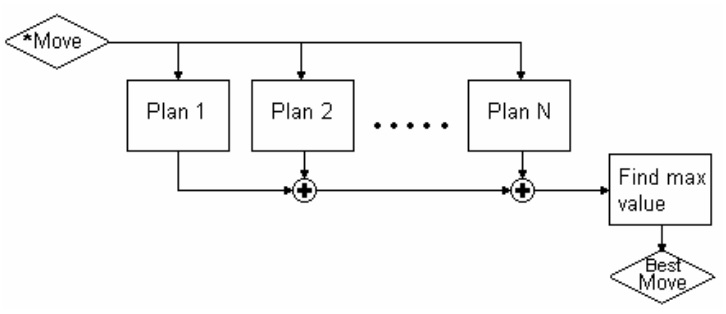
\includegraphics[scale=0.5]{plan.jpg}
  \caption{Finding the best move. [2]}
  \label{fig:plans1}
\end{figure}

\subsubsection{Invincible - Results}

Invincible held his own against a varied set of opponents, winning three out of five games. It lost the first one comfortably because of the lack of experience. 
It won the next three games playing more aggressively, capitalizing on human unfamiliarity, and retaining its lead. 
It lacked the ability to detect the weakness of unusual approaches like the one used in the fifth game. 
It can never be told everything so there will always be situations that it can’t handle correctly. 
The idea of using pre-defined plans worked to a degree but it will not be able to defeat high level opponents due to the logic behind pre-generated plans. 

\section{Nash Equilibrium Stratego Bots}

Stratego is an example of a two-player zero-sum imperfect information game. Each player has their own policy $\pi_i$, which can be switched at any point during the game (episode). Stratego is a zero-sum game because the sum of the rewards between all players for a given action is 0. Since Stratego is a two-player game, this means that a player receiving a reward $r$ means the other player receives a reward $-r$. A set of policies is in Nash equilibrium if no player can change their current policy to receive a higher reward. This effectively gives an ideal strategy for a given player in a game, so many Stratego bots are based on finding a Nash equilibrium. 

\subsection{ReBeL}

ReBeL (Recursive Belief-Based Learning) is an algorithm created by Facebook’s AI Research team in 2020, which is designed to converge to the Nash equilibrium of a two-player zero-sum game. 
ReBeL is an example of an RL+Search algorithm, which simulates intuition by searching the game tree to look ahead in the game and neural networks to make judgments on the value of states to make its next decision. 
Unlike previous RL+Search algorithms --- such as AlphaZero --- ReBeL is capable of handling imperfect information games. The ReBeL algorithm has been adapted to play a variant of Stratego called Stratego Tiny, which is played on a 4x4 board with 4 pieces per player. [4]

To handle imperfect information, we can model this information using \textbf{infostates} and \textbf{infosets}. An infostate for a player $i$ is the set of states that cannot be distinguished with the information that player $i$ has. 
An infoset for a player $i$ is an infostate where it is player $i$’s turn to make an action. Strategies for both players are made with respect to their infosets. 
ReBeL also relies on a public belief state, which is a probability distribution over the histories (nodes in the game tree) that the game could be in. 
As more information is revealed, the public belief state is updated accordingly. [5]

\subsubsection{Counterfactual Regret Minimization}

Counterfactual Regret Minimization (CFR) is an algorithm that can solve the Nash equilibrium for an imperfect information game. However, it is too slow to use on its own as it requires searching the entire game tree to find the Nash equilibrium. 
For a game like Stratego, with a game tree of size $10^{535}$, it’s impractical to use the algorithm alone. Instead, it is used for the search part of RL+Search, up to a given depth of the game-tree. [5]

CFR is built on the idea of regret, which quantifies the desire to have taken another action instead of the current action that was taken. Positive regret means that the other action is prefered over the current action. 
Formally, the \textbf{counterfactual regret} for not taking an action $a$ at infoset $I_i$ under policy $\pi$, is defined as $$ r^{\pi}_i(I_i)(a) = v_i^{\pi_{I_i \rightarrow a}}(I_i) - v_i^{\pi}(I_i) $$ 
Additionally, we define the \textbf{counterfactual regret-sum} for action $a$ at iteration $t$, for infoset $I_i$ under policy $\pi$ as $$ R_i^t(I_i)(a) = \sum_{\tau = 1}^t r_i^{\pi^\tau}(I_i)(a) $$ 

Running over $t$ iterations, the algorithm computes the regret-sum for a player $i$, then defines a new policy where actions with only positive regret are taken, weighted based on regret. 
After the $t$ iterations are complete, the average of the policies is taken. This averaged policy approaches Nash equilibrium as $t \rightarrow \infty$. 

\subsubsection{ReBeL itself}

\begin{table}
  \caption{Parameters used to train ReBeL [5]}
  \label{rebel-train}
  \centering
  \begin{tabular}{ll}
    \toprule
    Bot name	& Description \\ \midrule
    d3\_100	& ReBeL trained on all the data, playing with CFR-depth 3 \\
    d3\_50	& ReBeL trained on the first 50\% of the data, playing with CFR-depth 3 \\
    d3\_25 	& ReBeL trained on the first 25\% of the data, playing with CFR-depth 3 \\
    d2\_100 	& ReBeL trained on all the data, playing with CFR-depth 2 \\
    cfr\_d3 	& CFR with evaluation of non-terminal nodes to 0 and playing with depth 3 \\
    random 	& Chooses actions uniformly at random among the valid actions \\
    \bottomrule
  \end{tabular}
\end{table}

\begin{table}
  \caption{ReBeL tournament results [5]}
  \label{rebel-results}
  \centering
  \begin{tabular}{ccccccc}
    \toprule
    P1/P2 & d3\_100 & d3\_50 & d3\_25 & d2\_100 & cfr\_d3 & random \\
d3\_100 & - & 98/154/4 & 122/129/5 & 190/45/21 & 136/120/0 & 237/19/0 \\
d3\_50 & 153/97/6 & - & 142/113/1 & 203/47/6 & 174/79/3 & 245/9/2 \\
d3\_25 & 187/69/0 & 154/101/1 & - & 203/51/2 & 182/74/0 & 252/2/2 \\
d2\_100 & 70/175/11 & 66/181/9 & 62/194/0 - & 85/171/0 & 204/51/1 \\
cfr\_d3 & 132/124/0 & 133/123/0 & 110/146/0 & 179/77/0 & - & 245/11/0 \\
random & 36/220/0 & 30/226/0 & 15/241/0 & 55/198/3 & 37/219/0 & - \\
    \bottomrule
  \end{tabular}
\end{table}

ReBeL is trained in belief representation, based on the public belief state. A subgame is constructed with the root at the current state of the game. This game is solved to a certain depth using CFR. 
The value of each leaf in the game tree is estimated based on the infostate and the belief state with respect to the current policy as input to a neural network.  
ReBeL was trained with no outside input, relying on self-play to generate the values for each action. Various versions of ReBeL were trained based on CFR depth and percentage of information kept during training. (See Table~\ref{rebel-train})

There are 3 things to note from the results (See Table~\ref{rebel-results}). The first is that the player to move first (Player 1) appears to have an advantage compared to other player, winning a larger percentage of games. 
The second is that larger CFR depths resulted in a higher win rate. This makes sense since this provides more information to make a decision. The third is that more data kept during training did not result in a higher win rate. 
This was unexpected for the author, and they posit that the reason behind this is that the data was somehow overfitting, leading to a more inaccurate network. 

One issue with ReBeL is that it doesn’t scale well. As the game tree grows, running CFR search becomes more costly, to the point of infeasibility. 
Since Stratego Tiny is smaller than the actual Stratego, it’s unlikely that this method will be as effective when applied to Stratego. 

\subsection{Pipeline Policy Space Response Oracles}

Policy Space Response Oracles (PSRO) are a class of algorithms that find an approximate Nash equilibrium for normal-form games. A \textbf{normal-form game} is a tuple $(\Pi, U)$ where $\Pi$ is the set of strategies for each player and $U$ is the table of payoffs (rewards) for each player’s policy. 
\textbf{Extensive-form games} contain more information about the game, such as turn-taking. Stratego is an example of an extensive-form game. 
Extensive-form games can be reduced to normal-form games for the purpose of solving Nash equilibrium. 
In theory, this would be bad, since turning an extensive-form game into a normal-form game increases the policies exponentially. In practice, this doesn’t make a big difference in performance. [6]

\subsubsection{Double Oracle Algorithm}

The Double Oracle algorithm works by keeping a subset of policies at a given iteration, then finding a Nash equilibrium of those policies. 
Once that’s been done, a policy is computed for each player to exploit this Nash equilibrium and is added to the set of policies being analyzed. 
PSRO approximates the Double Oracle algorithm by having each policy play each other and keeping track of the utility in a matrix. 
Then, an RL algorithm is used to compute a response to the Nash equilibrium. The issue with this algorithm is the sequential nature of it; only one policy is being computed at a given time. 
This is what the current paper addresses. 

\subsubsection{Pipeline PSRO}

\begin{table}
  \caption{Barrage P2SRO Results [6]}
  \label{p2sro-results}
  \centering
  \begin{tabular}{lc}
    \toprule
    Name		& P2SRO Win Rate vs. Bot \\ \midrule
    Asmodeus		& 81\% \\
    Celsius		& 70\% \\
    Vixen		& 69\% \\
    Celsius1.1 	& 65\% \\
    \textbf{All Bots Average} 	& \textbf{71\%} \\
    \bottomrule
  \end{tabular}
\end{table}

Pipeline PSRO (P2SRO) is a variant of PSRO that computes multiple policies at once in parallel, increasing the speed at which an approximate Nash equilibrium is reached. 
P2SRO splits the policies used into two sets: \textbf{fixed} and \textbf{active}. Fixed policies aren’t being actively trained anymore but are still part of the set of policies. 
Active policies are being trained on all the policies lower than them in the pipeline. Once the lowest active policy reaches a training threshold, it becomes fixed, and a new active policy is added to the end of the pipeline. 
This algorithm lets multiple policies be trained at once and gives new active policies a head start, since they are trained on lower active policies in the pipeline.

An implementation of P2SRO was created with fictitious self-play used to calculate the Nash equilibrium of the current policies and the discrete-action version of Soft Actor-Critic used to find the best response policy. 
This implementation played Barrage Stratego, which is played on the same 10x10 board as regular Stratego, but with 8 pieces instead of 40.  
It was tested against various known Stratego bots that can play Barrage Stratego, including some that won past Computer Stratego Championships. 
After 820,000 episodes, the implementation had a win rate of around 71\% against other bots (See Table~\ref{p2sro-results}). 

\subsection{DeepNash}

DeepNash is a bot created by DeepMind (a subsidiary of Alphabet) designed to play imperfect information games such as Stratego. 
DeepNash relies on an algorithm called Regularized Nash Dynamics (R-NaD) and a deep neural network to achieve an approximate Nash equilibrium. 
This approach is model-free, meaning the beliefs of the opponent aren’t modelled when finding the Nash equilibrium. [7]

\subsubsection{Regularized Nash Dynamics}

R-NaD is a game-theoretic algorithm that evolves a policy with high fitness in a dynamic environment that allows it to converge to a Nash equilibrium. 
R-NaD is comprised of three steps: reward transformation, dynamics, and update. \textbf{Reward transformation} modifies the rewards of the game using a regularization policy. 
$$ r^i(\pi^i, \pi^{-i}, a^i, a^{-i}) = r^i(a^i, a^{-i}) - \eta\log(\frac{\pi^i(a^i)}{\pi_{reg}^i(a^i)}) + \eta\log(\frac{\pi^{-i}(a^{-i})}{\pi_{reg}^{-i}(a^{-i})})$$ 
The regularization constant $\eta$ affects how fast the dynamics converge to a fixed point but increases the number of iterations (fixed points) needed to approach a Nash equilibrium. 
The \textbf{dynamics} step evolves the system based on replicator dynamics (which is similar to a regret minimization algorithm known as Follow the Regularized Leader) and is defined as 
$$ \frac{d}{d\tau} \pi_\tau^i (a^i) = \pi_\tau^i (a^i) [Q_{\pi_\tau}^i(a^i) - \sum_{b^i} \pi_\tau^i (b^i) Q_{\pi_\tau}^i(b^i)]$$ 
This dynamics system has a fixed point that it converges to, which represents a policy. This policy is used in the \textbf{update} step, where it becomes the next regularization policy, and the next iteration occurs. 

\subsubsection{DeepNash itself}

\begin{table}
  \caption{DeepNash Results [7]}
  \label{deepnash-results}
  \centering
  \begin{tabular}{lc|rrr}
    \toprule
    Opponent			& Number of Games 	& Wins & Draws & Losses\\ \midrule
    Probe			& 30	& 100.0\%	& 0.0\%	& 0.0\% \\
    Master of the Flag	& 30	& 100.0\%	& 0.0\%	& 0.0\% \\
    Demon of Ignorance	& 800	& 97.1\%	& 1.8\%	& 1.1\% \\
    Asmodeus			& 800	& 99.7\%	& 0.0\%	& 0.3\% \\
    Celsius			& 800	& 98.2\%	& 0.0\%	& 1.8\% \\
    Celsius1.1 		& 800	& 97.9\%	& 0.0\%	& 2.1\% \\
    PeternLewis		& 800	& 99.9\%	& 0.0\%	& 0.1\% \\
    Vixen			& 800	& 100.0\%	& 0.0\%	& 0.0\% \\
    \bottomrule
  \end{tabular}
\end{table}

DeepNash implements R-NaD using deep learning. The dynamics step of R-NaD is implemented in two parts: using a $v$-trace estimator to estimate the value function for the system, and Neural Replicator Dynamics (NeuRD); 
a policy gradient algorithm that modifies the softmax policy gradient to find the fixed point in the dynamic system. [8] 
The implementation was also fine-tuned at the end, to avoid annoying sequences of actions (e.g., moving one piece back and forth) for human players, as well as to avoid actions with sufficiently low probabilities. 

DeepNash was tested on both humans and bots in the full Stratego game. DeepNash played 50 ranked matches on the Gravon website, winning 42 of them, and placing 3\textsuperscript{rd} overall on the website's leaderboard. 
Against bots, DeepNash played up to 800 games against various leading Stratego bots and won over 95\% of them (See Table~\ref{deepnash-results}). 

\section{Conclusion}
When comparing the data-driven approaches to the Nash equilibrium approaches for Stratego, the Nash equilibrium approaches appear to outperform the data-driven approaches. 
This is likely due to the nature of imperfect information games. The lack of information causes bluffing and deception to be a core part of the games, requiring some amount of novelty in play. 
Rigid approaches defined by data do not have the flexibility needed to perform these tasks at a high level for a game as complex as Stratego, whereas the Nash equilibrium approaches are formed using self-play, allowing for the necessary flexibility to arise naturally. 

Among the Nash equilibrium approaches ReBeL is unable to scale for larger problems, which makes it an issue for practical applications.  
Between P2SRO and DeepNash, while they haven’t played against each other, they have played against similar bots, and in that respect, DeepNash comes out on top. 
However, this may be due to DeepMind, the creators of DeepNash, having more funding and computing power compared to the researchers who made P2SRO. 
For further research, comparing P2SRO against DeepNash seems like a good approach. Getting some human tests against P2SRO would also help make a fairer comparison. 
Lastly, it would be interesting to see how DeepNash fares against top players in the Stratego World Championship, to see if it can surpass the top human players. 

\section*{References}

\small

[1] Stankiewicz, J. A., \& Schadd, M. P. (2009). Opponent modeling in stratego. \textit{Natural Computing}.

[2] de Boer, V., Rothkrantz, L. J., \& Wiggers, P. (2008). Invincible-A Stratego Bot. \textit{International Journal of Intelligent Games \& Simulation}, 5(1).

[3] Redeca, S., \& Groza, A. (2018, September). Designing agents for the Stratego game. In \textit{2018 IEEE 14th International Conference on Intelligent Computer Communication and Processing (ICCP)} (pp. 97-104). IEEE.

[4] Brown, N., Bakhtin, A., Lerer, A., \& Gong, Q. (2020). Combining deep reinforcement learning and search for imperfect-information games. \textit{Advances in Neural Information Processing Systems}, 33, 17057-17069.

[5] Falk, A. (2021). Stratego Using Deep Reinforcement Learning and Search.

[6] McAleer, S., Lanier, J. B., Fox, R., \& Baldi, P. (2020). Pipeline psro: A scalable approach for finding approximate nash equilibria in large games. \textit{Advances in neural information processing systems}, 33, 20238-20248.

[7] Perolat, J., De Vylder, B., Hennes, D., Tarassov, E., Strub, F., de Boer, V., ... \& Tuyls, K. (2022). Mastering the game of Stratego with model-free multiagent reinforcement learning. \textit{Science}, 378(6623), 990-996.

[8] Hennes, D., Morrill, D., Omidshafiei, S., Munos, R., Perolat, J., Lanctot, M., ... \& Tuyls, K. (2019). Neural replicator dynamics. \textit{arXiv preprint arXiv}:1906.00190.

\section*{Appendix}

\begin{enumerate}
  \item Advantage: “Unlimited” search depth: The search depth is unlimited because the depth is defined by the useful depth to detect and complete a plan. 
  Because of the directional rather than exhaustive search this depth can easily be reached. 
  This is a relatively small search problem that can easily be performed thousands of times without noticeable delay on modern hardware 
  \item Advantage: Possibilities to bluff: Bluffing can be implemented by defining what makes moves good for bluffing. Usually this means performing a normal plan with the wrong pieces. 
  If “Invincible” can find a piece of which the opponent may believe it is the right piece for a certain plan and he uses it for that plan, then the opponent's belief that this piece has a rank when in reality it doesn’t have is strengthened. 
  This behavior is easy to implement when moves are chosen based on plans but very hard/impossible to include in a system that finds all the effects of a limited sequence of moves. 
  \item Advantage: Possibilities to coordinate attacks with multiple pieces: 
  There are not many things in Stratego that a single piece can do, but plans that require multiple pieces generally also require many more moves. 
  An exhaustive search of 12 plies allows to find plans that require 1 piece to move 6 fields, or 2 pieces to move 3 fields. 
  That means both pieces must be already very close to where they are needed before a combination that requires these pieces can be found. 
  If this is defined as a plan, then this plan can find the location of the required pieces and guide them where they have to be also as a search over a 10x10 graph. 
  \item Advantage: Focus computation on interesting situations: 
  The computational is used more specifically for computing interesting aspects of a board position rather than for computing all the possible move sequences, out of which most are not going to be interesting 
  \item Disadvantage: “Invincible” knows only what it is told: Because there is no exhaustive search, everything that is not formulated as a plan will be completely ignored. 
  If there is no plan telling “Invincible” to move a known low piece away when a known higher piece is approaching it then it will not do so. 
  There is however only a limited number of useful things to pay attention to on short-term planning, and since the long-term plans can’t be seen by exhaustive search anyway this is only a disadvantage 
  in terms of programming time and not in playing strength 
  \item Disadvantage: Comparable information is calculated multiple times: Many plans use similar information, but can’t use each others results if the calculation is split in independent sub-problems. 
  This means that sometimes the same calculation is done multiple times. This is of course inefficient, but because time isn’t really an issue this doesn’t prove to be a big problem 
  \item Disadvantage: Game specific knowledge needed: So much of the search can be ignored only because of knowledge specific to the domain (in this case the game Stratego). 
  A human expert in the domain will have to decide which plans should be added. In either case, a lot of the development time will go into formalizing human experience into computer-readable algorithms 
\end{enumerate}

\end{document}
